\section{Results}

\subsection{Multiplying two matrices with different sizes}\label{subsec:res-sizes}
This section discusses the time taken both for parallelized and single thread  multiplying two matrices of the same size.
This test repeated the multiplication with the size of the matrix increasing each time from a size of 2 to a size of 200.
Both the single thread and parallel programs were run 20 times per size and an average was taken for maximum accuracy
The results of the multiplication are shown in figure \ref{fig:Single_thread_vs_Parallel_processing_time}.

\begin{figure}[H]
    \centering
    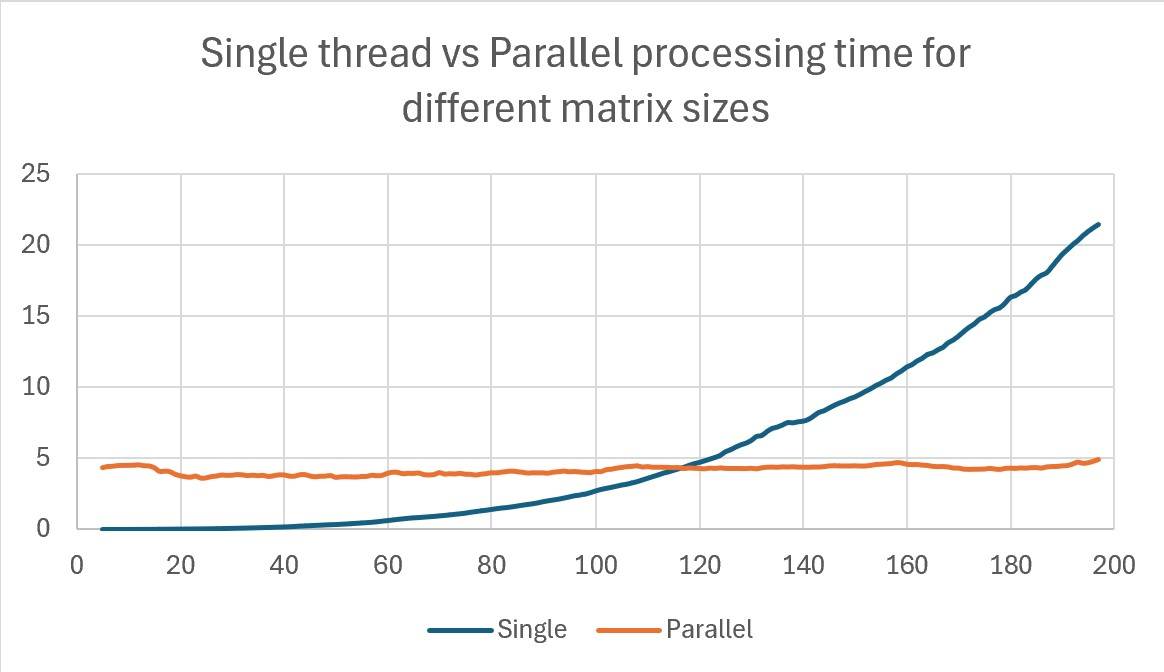
\includegraphics[width=0.8\columnwidth]{Figures/Single_thread_vs_Parallel_processing_time_for_different_matrix_sizes}
    \caption{Graph of single thread vs Parallel processing time for different matrix sizes}
    \label{fig:Single_thread_vs_Parallel_processing_time}
\end{figure}

The results in \ref{fig:Single_thread_vs_Parallel_processing_time} clearly show that the time taken for single threaded matrix multiplication is initially faster than parallelized multiplication up to size of the matrix but after a certain threshold the parallelized program becomes faster.
With the hardware used in this report, the threshold was roughly at size 100.


It can be seen that both graphs appear to follow an exponential or power trend, with the parallel program having a much lower gain than the single thread program.
Additionally, the single thread program times appears to start at close to 0 ms for the smallest matrix size while the parallel program times appear to start at around 4 ms.
This is due to the time required to set up the parallel program is 4 ms which is longer than that of the single thread program.


However, as the matrix size increases, the time taken for single thread program increases at a faster exponential rate compared to that of the parallel program, resulting in the parallel program eventually overtaking the single thread program.

\subsection{Multiplying different numbers of matrices of the same size}
This section discusses the time taken for parallelized verses single thread multiplying different numbers of matrices of the same size.
Each test was conducted on a different matrix size (5, 10, 20, 50 or 100) and was run with a matrix count of 5 to 45.
Both the single thread and parallel programs were run 20 times per count and an average was taken for maximum accuracy

\begin{figure}[H]
    \centering
    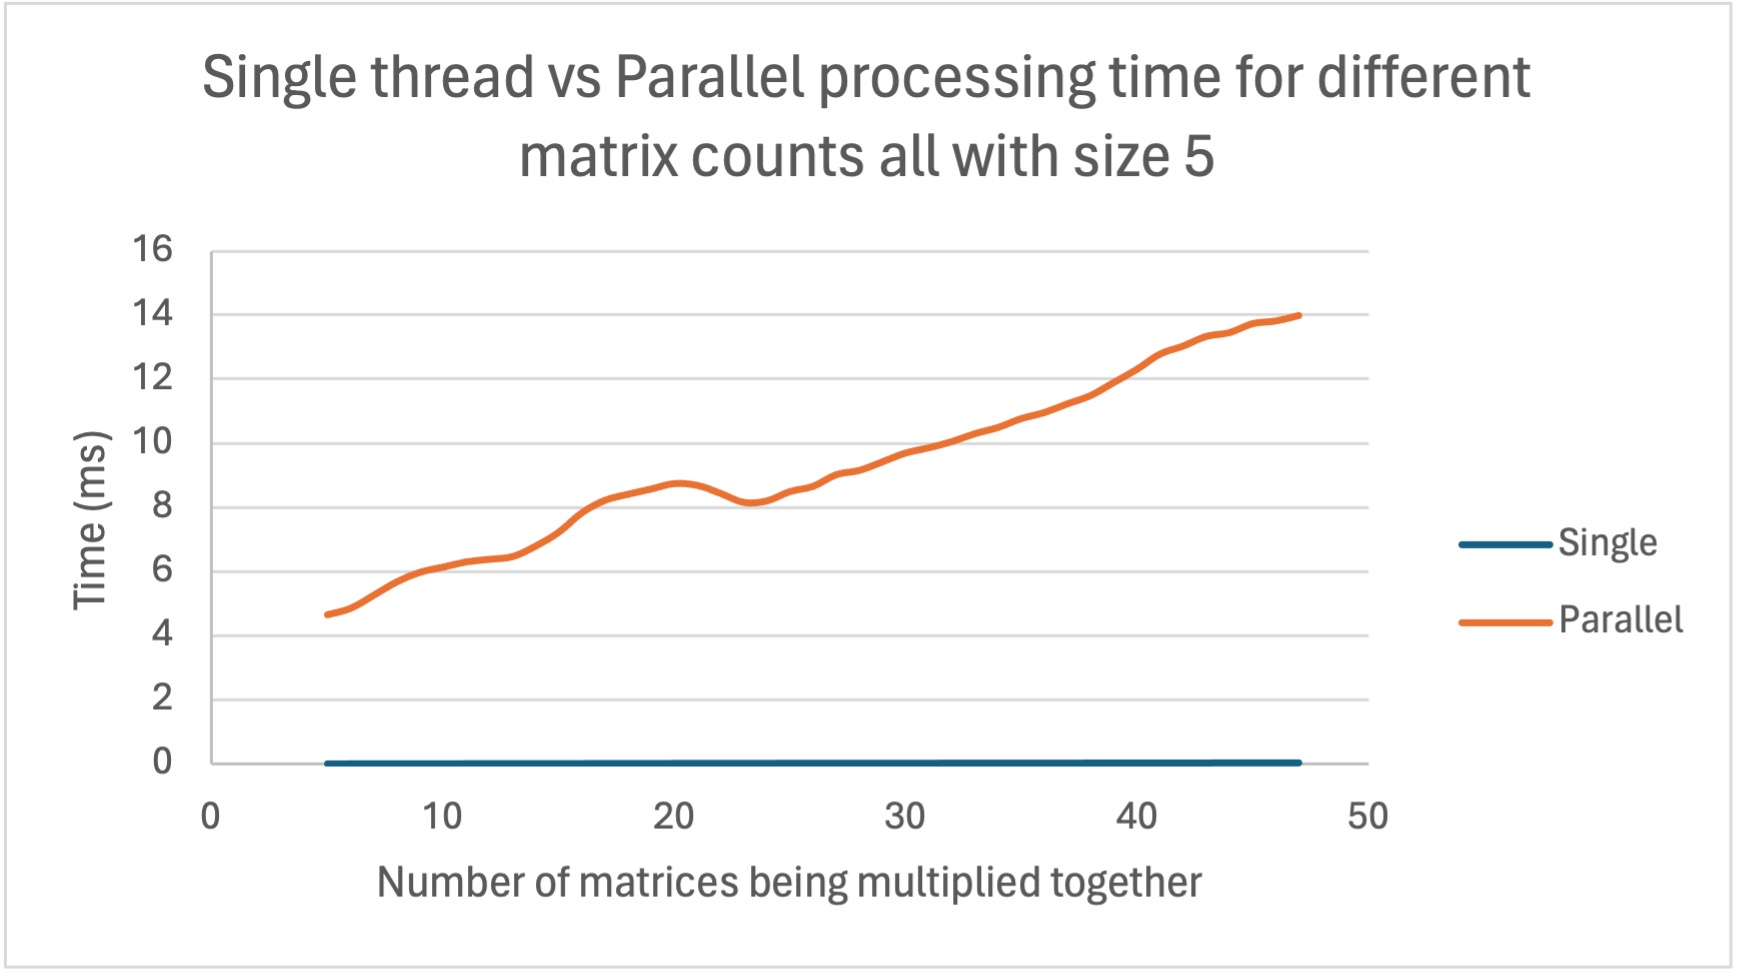
\includegraphics[width=0.8\columnwidth]{Figures/different_matrix_counts_size_5}
    \caption{Single thread vs Parallel processing time for different matrix counts all with size 10}
    \label{fig:different_matrix_counts_size 5}
\end{figure}

\begin{figure}[H]
    \centering
    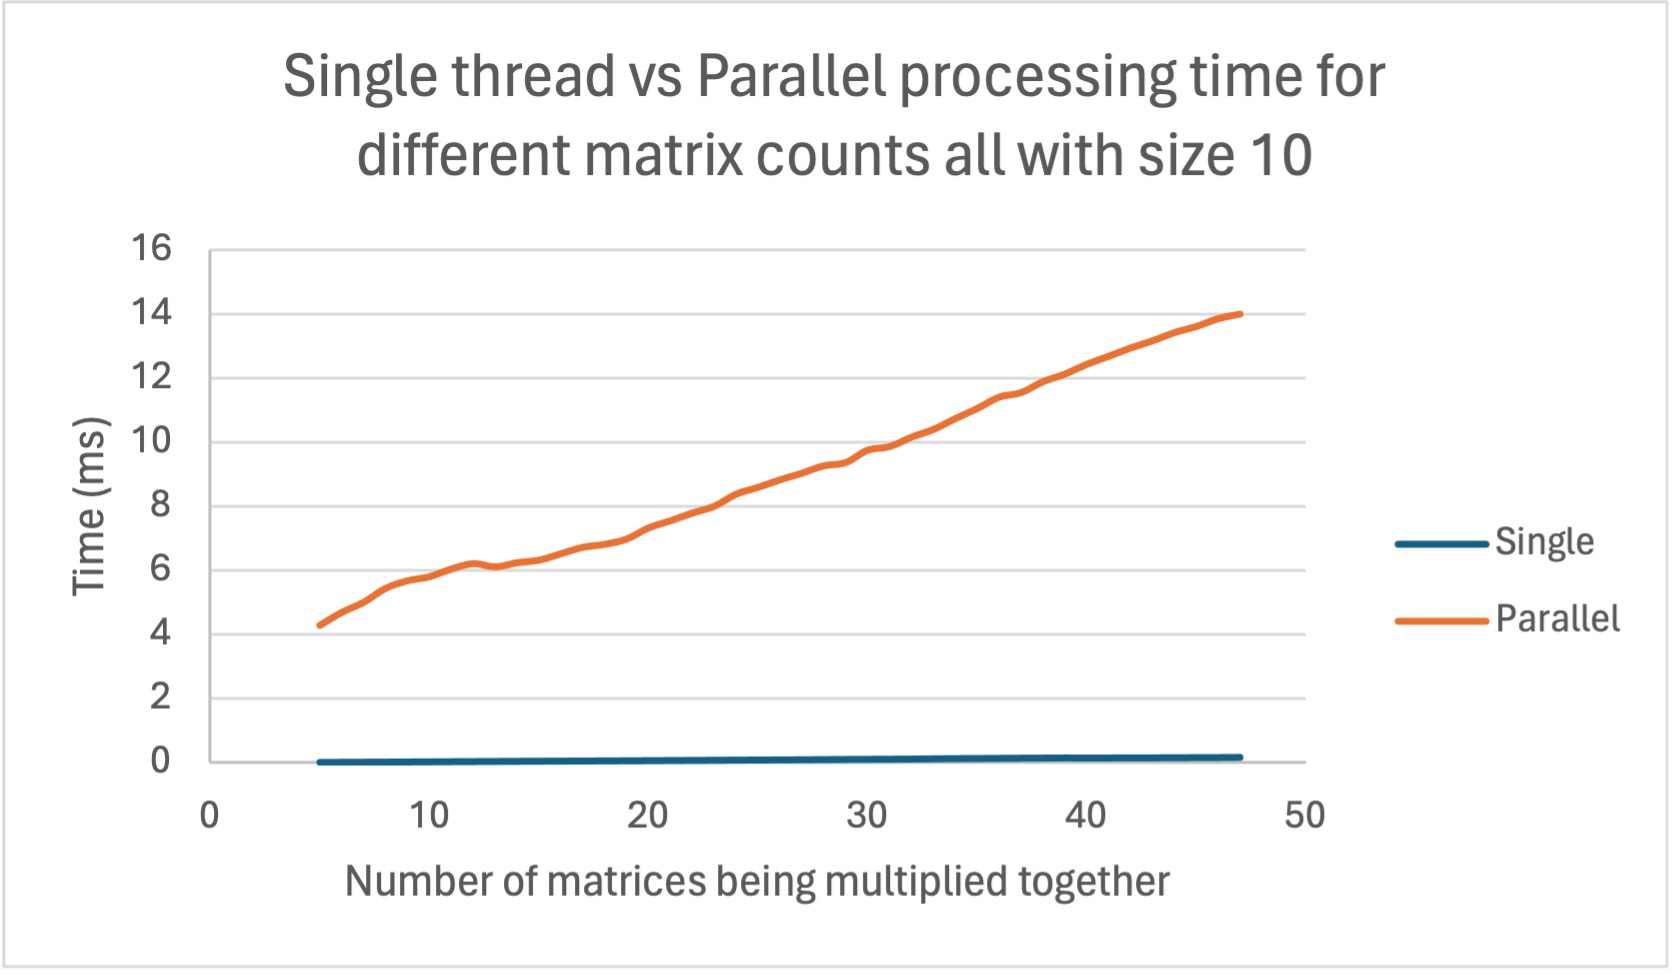
\includegraphics[width=0.8\columnwidth]{Figures/different_matrix_counts_size_10}
    \caption{Single thread vs Parallel processing time for different matrix counts all with size 10}
    \label{fig:different_matrix_counts_size 10}
\end{figure}

\begin{figure}[H]
    \centering
    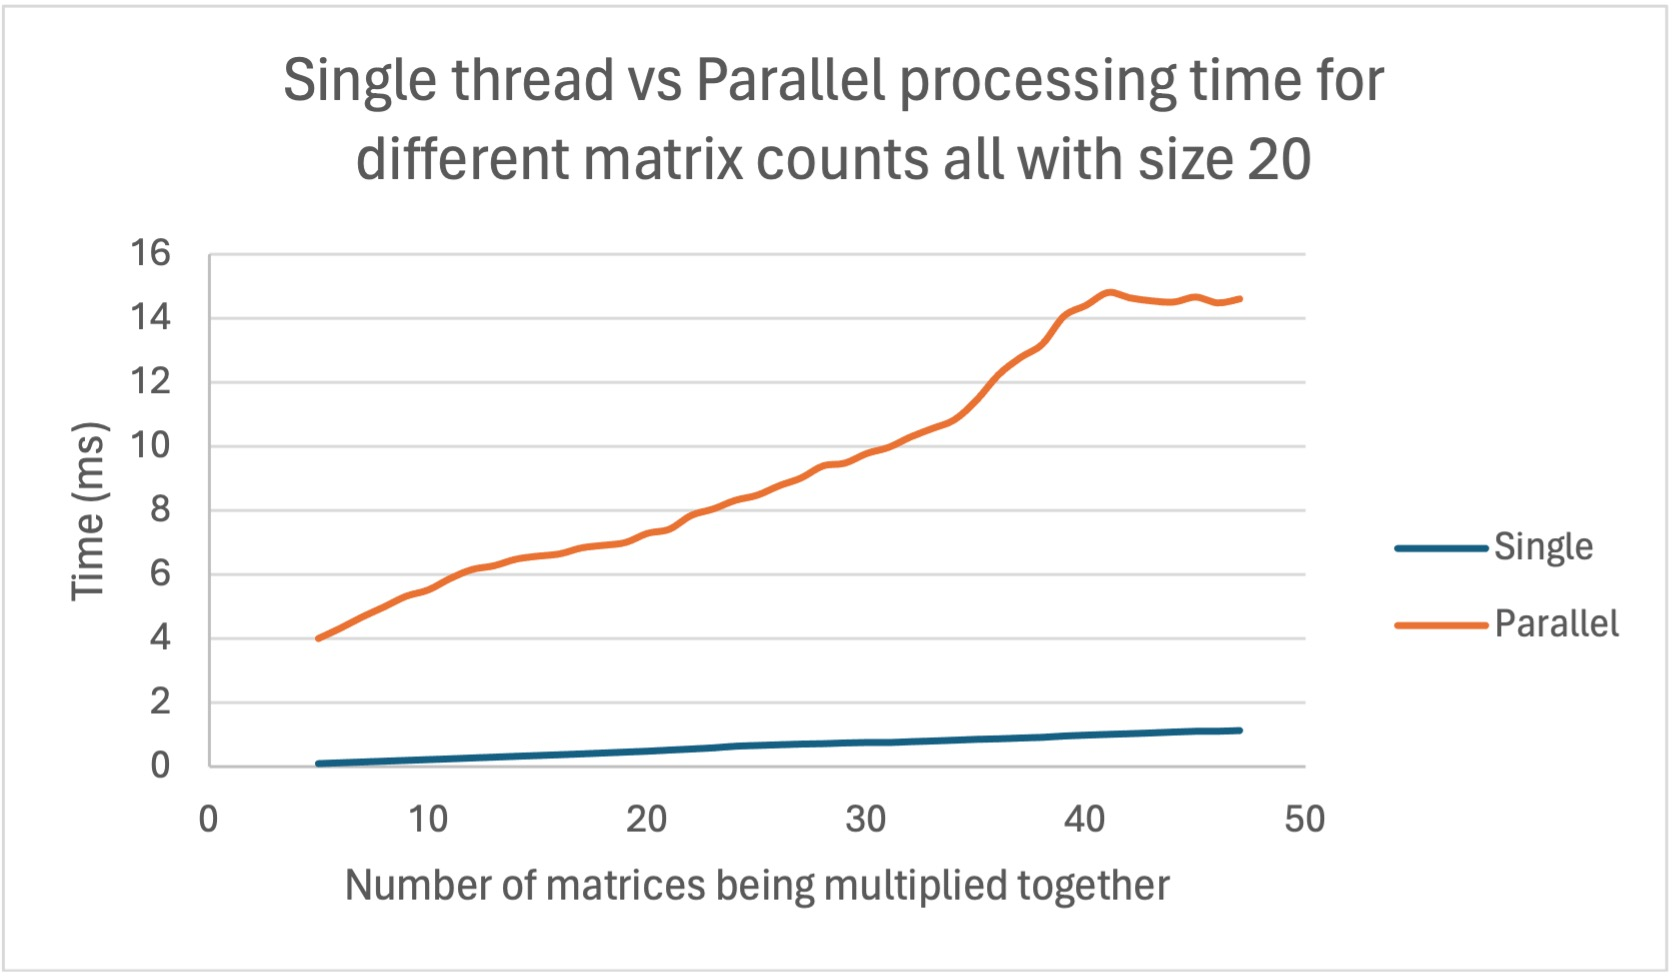
\includegraphics[width=0.8\columnwidth]{Figures/different_matrix_counts_size_20}
    \caption{Single thread vs Parallel processing time for different matrix counts all with size 20}
    \label{fig:different_matrix_counts_size 20}
\end{figure}

\begin{figure}[H]
    \centering
    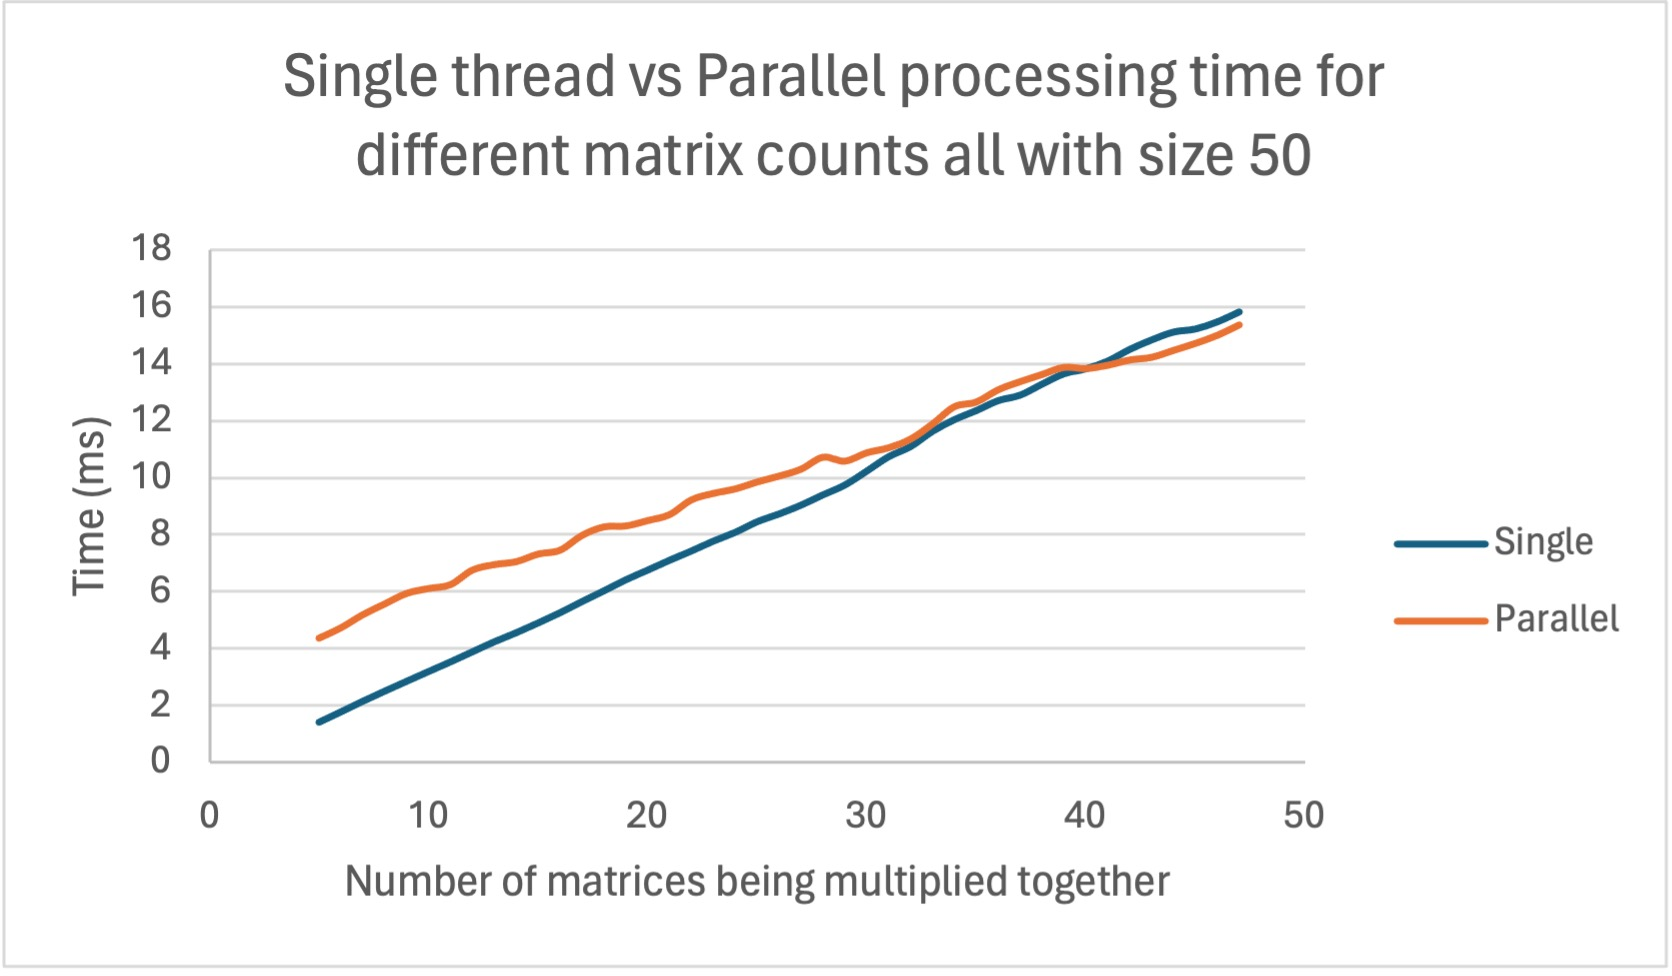
\includegraphics[width=0.8\columnwidth]{Figures/different_matrix_counts_size_50}
    \caption{Single thread vs Parallel processing time for different matrix counts all with size 50}
    \label{fig:different_matrix_counts_size 50}
\end{figure}

\begin{figure}[H]
    \centering
    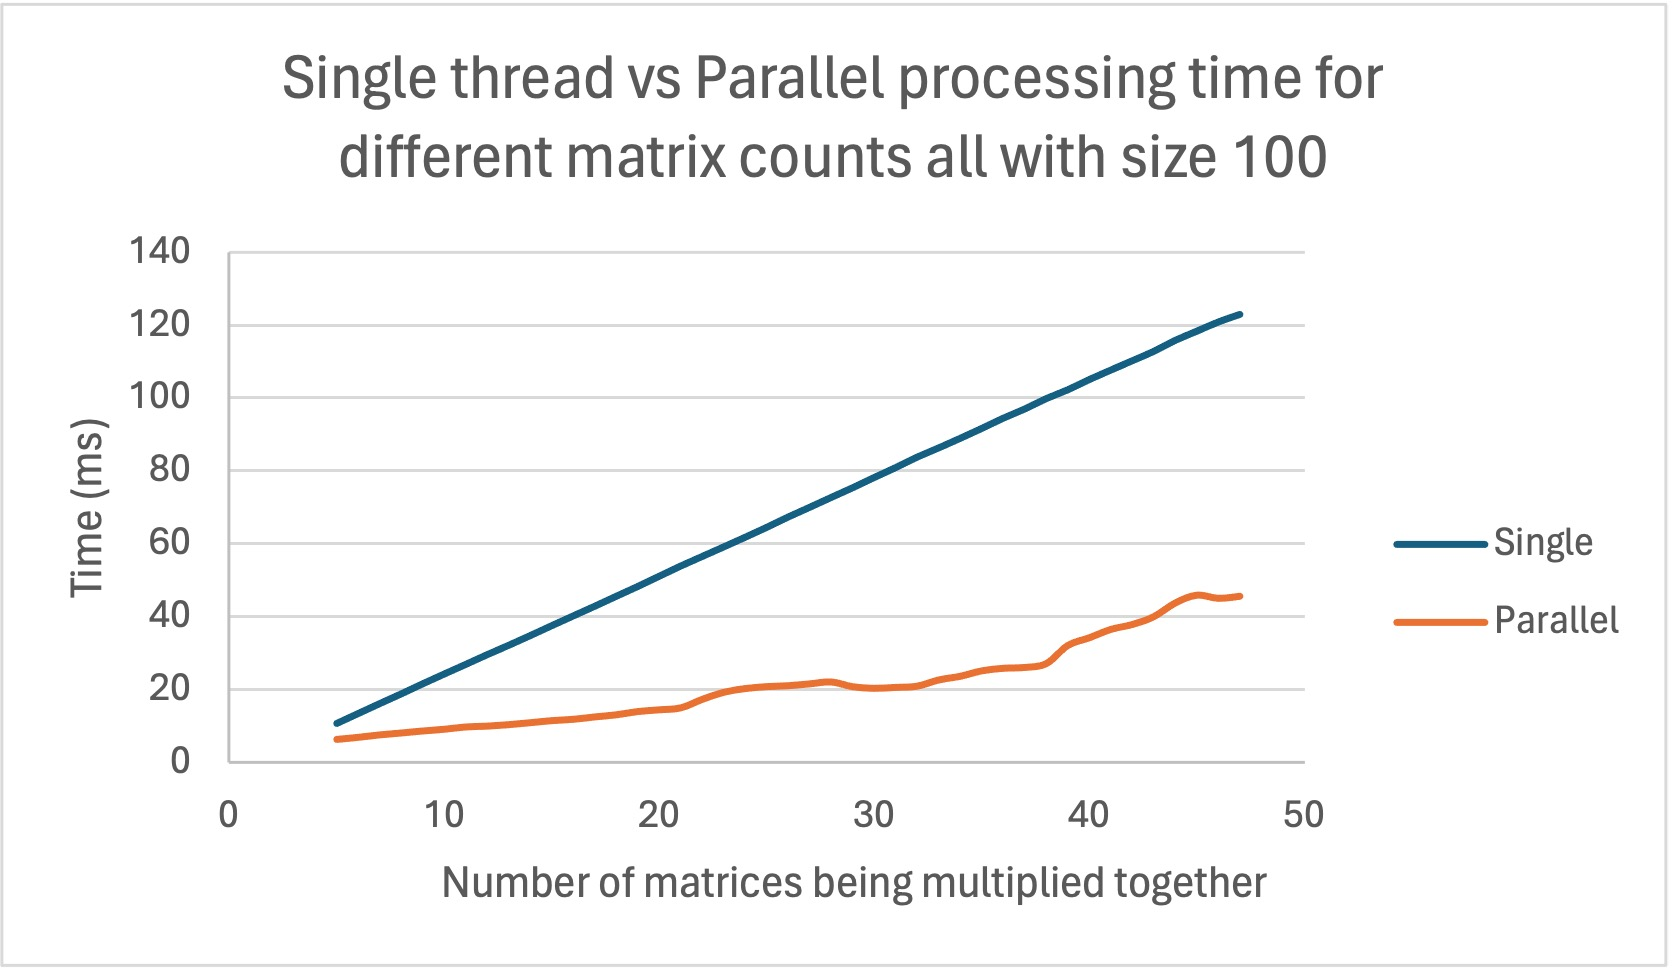
\includegraphics[width=0.8\columnwidth]{Figures/different_matrix_counts_size_100}
    \caption{Single thread vs Parallel processing time for different matrix counts all with size 100}
    \label{fig:different_matrix_counts_size 100}
\end{figure}

Looking at the results in figures: \ref{fig:different_matrix_counts_size 5}, \ref{fig:different_matrix_counts_size 10}, \ref{fig:different_matrix_counts_size 20}, \ref{fig:different_matrix_counts_size 50} and \ref{fig:different_matrix_counts_size 100},
it can be seen that both the single and parallel programs' time follow an approximate linear trend and that the parallel program has an initial overhead of around 5 ms with a matrix count of 5.
While the graphs cannot extend to where zero matrices are multiplied together, they can be extrapolated to show that the parallel program always has an initial overhead that is significantly higher than the single thread program, even in figure \ref{fig:different_matrix_counts_size 100}.


It should be noted that the overhead for the parallel program can be broken up into to parts: the overhead of setting up the OpenCL device and programs and the overhead of starting each instance of the kernel program.
The latter, in conjunction with the runtime of the kernel program itself, occurs once per matrix multiplication and is the reason that the parallel program's time follows a linear trend.
By extension, the single threaded program also follows a linear trend for similar reasoning.


It also should be noted that the speed of the parallel program increases compared to the single thread program as the matrix count increases and as the matrix size increases.
The speed up with the increase of matrix count is due to the same reasoning as in the first test, where the single thread program's time increases at a fast rate eventually allowing for the parallel program to overtake it.
This is shown in figure \ref{fig:different_matrix_counts_size 50} where the threshold point was around 40 matrices of size 50x50 being multiplied together.


The speed up with increasing matrix sizes, which is the more significant in this test, is due to the percentage of parallelism in the parallel program increasing as the matrix size increases.
The increase in parallelism in due to the parallel program has three parts as mentioned above: the OpenCl setup overhead which stays constant, the kernel starting overhead which scales linearly with matrix count, and the kernel program which scales exponentially with matrix size but still at a slower rate than the single thread program as shown in section \ref{subsec:res-sizes}.
These factors combined cause an increase in parallelism with increasing matrix size which causes the parallel program to become faster than the single thread program as the matrix count increases.


\subsection{Multiplying different numbers of matrices with different sizes}
This section is a combination of the two above which produces the graph shown in figure \ref{fig:2d}.
Both the single thread and parallel programs were run only run once as running an average of multiple tests on each node reduces the total number of unique nodes that can be tested using the same amount of time and resources, and using more data points is more valuable to this report.

\begin{figure}[H]
    \centering
    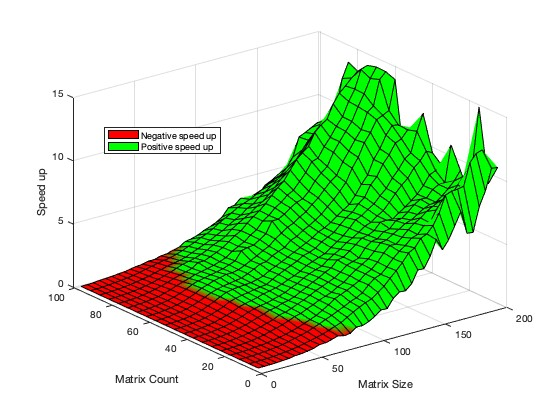
\includegraphics[width=1\columnwidth]{Figures/speedupsurf}
    \caption{A Surface plot showing the speed up from single thread to parallel matrix multiplication over different numbers of matrices of different size multiplied together}
    \label{fig:2d}
\end{figure}

This show that there is a clear threshold line of matrix size and matrix count where is it more efficient to parallelize matrix multiplication for any increase in either parameter.
With the hardware used in this report, the line extends roughly between 2 matrices of size 100x100 and 60 matrices of size 50x50 multiplied together.


The graph also indicates that for a very high number of matrices it suddenly become more efficient to use a single thread program which appears counter intuitive.
This could be due to 50 matrices of size 50x50 taking up too much space to be stored on the GPU cache on the hardware used in this report, and thus additional time is taken to transfer the data to the GPU cache; however further testing will be required to confirm this hypothesis.